% Slides accompanying "Learn RISC-V CPU Implementation and BSV" book
% Copyright (c) 2024 Rishiyur S. Nikhil, All Rights Reserved

% -*- mode: fundamental -*-

% Slides accompanying "Learn RISC-V CPU Implementation and BSV" book
% Copyright (c) 2024 Rishiyur S. Nikhil, All Rights Reserved

% This is a preamble shared by all the slide decks

\documentclass[10pt, aspectratio=169]{beamer}

% \documentclass[17pt]{beamer}

% Avail. font sizes: 8pt, 9pt, 10pt, 11pt, 12pt, 14pt, 17pt, 20pt.
% Default font size is 11pt (= 22pt in full screen mode).

\usepackage{verbatim}
\usepackage{fancyvrb}
\usepackage{listings}

% ================================================================
% Themes

\usetheme{Madrid}          % Line at bottom: Author (affiliation), OptTitle, Conf, page 

% \usetheme{Copenhagen}    % Same as Madrid except bottom line: Author, OptTitle

% \usetheme{Berkeley}    % Takes up 1-inch border on left and top

% ----------------
% colorthemes
% (default), beaver, beetle, seahorse, wolverine

\usecolortheme{seahorse}

% ================================================================
% Customization: show table of contents before each section
% Use \AtBeginSubsection    to show before each subsection

% \AtBeginSection[]
% {
%   \begin{frame}
%     \frametitle{Table of Contents}
%     \tableofcontents[currentsection]
%   \end{frame}
% }

% ================================================================

% ----------------
% The bsc compiler and BSV language
\newcommand{\bsc}{\emph{bsc}}
\newcommand{\BSV}{\bf{BSV}}
% ----------------
% ITALICISE WORDS
\newcommand{\ie}{\emph{i.e.,}}
\newcommand{\eg}{\emph{e.g.,}}
\newcommand{\Eg}{\emph{E.g.,}}
\newcommand{\etc}{\emph{etc.}}
\newcommand{\via}{\emph{via}}
\newcommand{\vs}{\emph{vs.}}

% ----------------
% EMPTY BOXES OF VARIOUS WIDTHS, FOR INDENTATION

\newcommand{\hm}{\hspace*{1em}}
\newcommand{\hmm}{\hspace*{2em}}
\newcommand{\hmmm}{\hspace*{3em}}
\newcommand{\hmmmm}{\hspace*{4em}}

% ----------------
% Convenient widths

\newlength{\hlessmm}
\setlength{\hlessmm}{\textwidth}
\addtolength{\hlessmm}{-2em}

\newlength{\hlessmmm}
\setlength{\hlessmmm}{\textwidth}
\addtolength{\hlessmmm}{-3em}

\newlength{\hlessmmmm}
\setlength{\hlessmmmm}{\textwidth}
\addtolength{\hlessmmmm}{-4em}

% ================================================================
% Title page

\title[Learn CPU design \& BSV]{Learn RISC-V CPU Implementation and BSV}

\subtitle{(BSV: a High-Level Hardware Design Language)}

\author[{\copyright} R.S.Nikhil]{Rishiyur S.~Nikhil}
% \institute{Bluespec, Inc.}

% Date is set differently in each slide deck

% \logo{
\includegraphics[height=0.6cm]{../Figures/Bluespec_Logo_2022-10}}

% End of preamble
% ****************************************************************


\date{L7: BSV: Modules and Interfaces}

% ****************************************************************

\begin{document}

% ================================================================

\begin{frame}
 \titlepage

 \begin{center}
  
\includegraphics[height=1cm]{Bluespec_Logo_2022-10}
 \end{center}

\end{frame}

% ================================================================

% -*- mode: fundamental -*-

% ================================================================

\begin{frame}[fragile]
\frametitle{Reminders}

\footnotesize

Please git clone: \url{https://github.com/rsnikhil/Learn_Bluespec_and_RISCV_Design} \\
(git pull for latest version).  Repsitory structure:

\vspace{1ex}

\begin{minipage}{0.5\textwidth}\scriptsize
\begin{Verbatim}[frame=single, numbers=left]
    ./Book_BLang_RISCV.pdf
      Slides/
          Slides_01_Intro.pdf
          Slides_02_ISA.pdf
          ...
      Exercises/
          Ex-03-A-Hello-World/
          Ex-03-B-Top-and-DUT/
          ...
      Code/
          src_Top/
          src_Drum/
          src_Fife/
          src_Common/
          ...
      Doc/Installing_bsc_Verilator_etc.{adoc,html}
\end{Verbatim}
\end{minipage}
\hm
\begin{minipage}{0.45\textwidth}
\begin{itemize}

 \item Slides and Exercise are numbered in sync with book Chapter numbers.

 \item For Exercises, please see Appendix E of the book.  Some (not
       all) exercises have associated code in the {\tt Exercises/}
       directory.

\end{itemize}
\end{minipage}

\vspace{2ex}

To compile and run the code for exercises, Drum and Fife, please make sure you have installed:

\begin{itemize}

 \item \emph{bsc} compiler (see \url{https://github.com/B-Lang-org/bsc})

 \item Verilator compiler (see \url{https://www.verilator.org/})
\end{itemize}

\footnotesize

\end{frame}

% ================================================================

\begin{frame}
\frametitle{Chapter Roadmap}

\footnotesize

\begin{center}
\frame{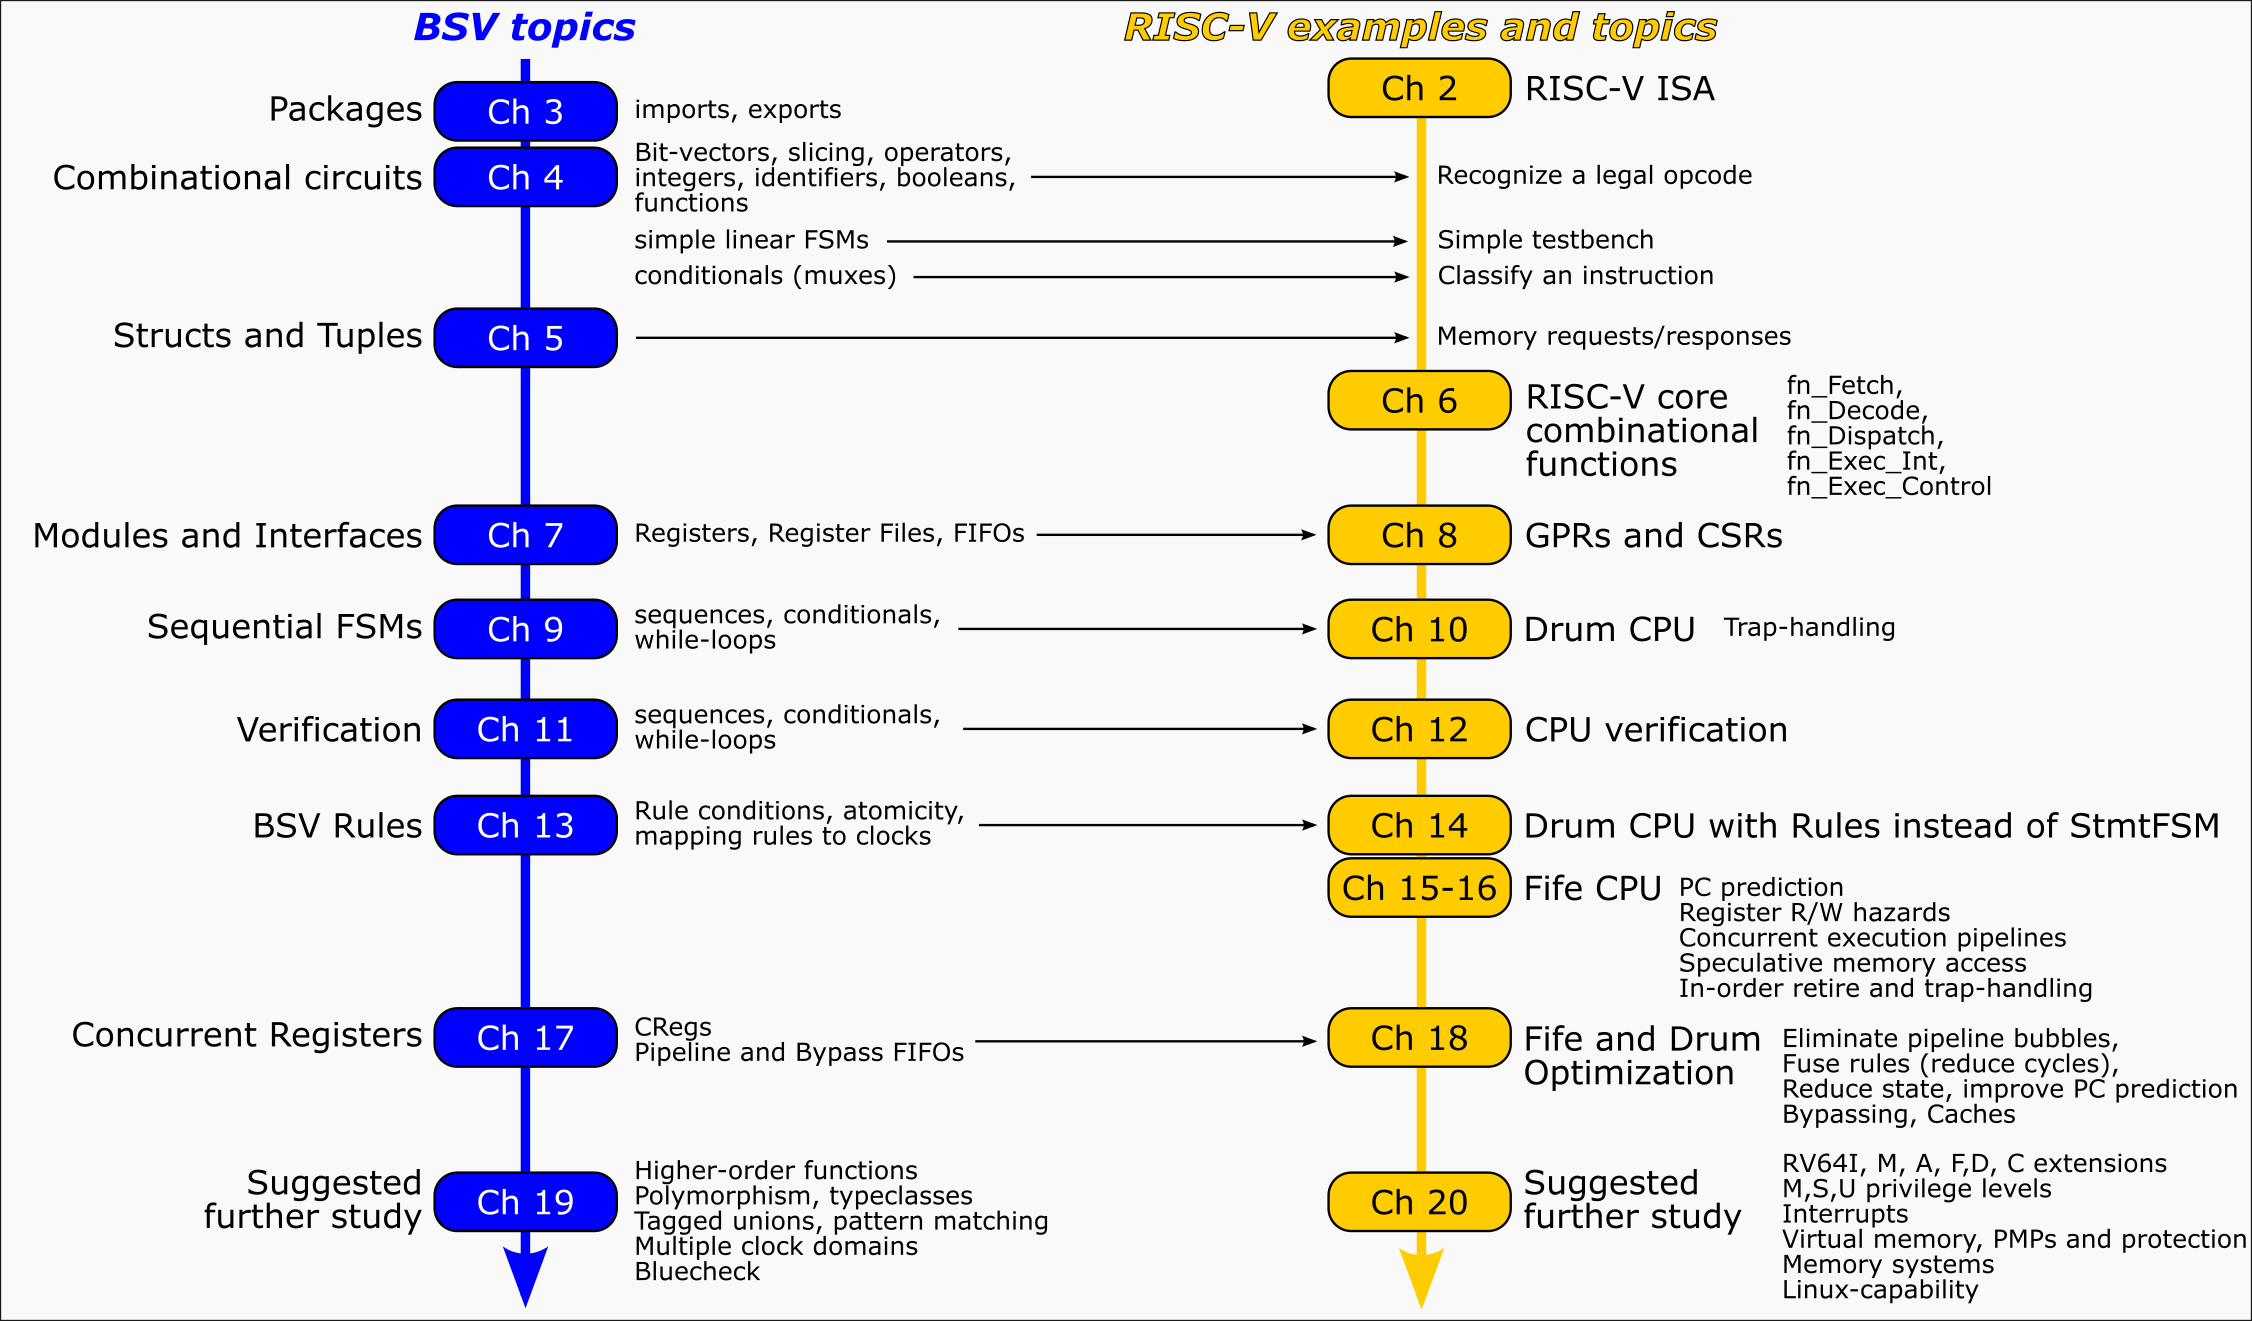
\includegraphics[height=0.825\textheight]{Fig_Chapter_Roadmap}}
\end{center}

\end{frame}

% ================================================================


% ================================================================

\begin{frame}
\frametitle{Flow of information between stages in Drum and Fife}

\footnotesize

\begin{center}
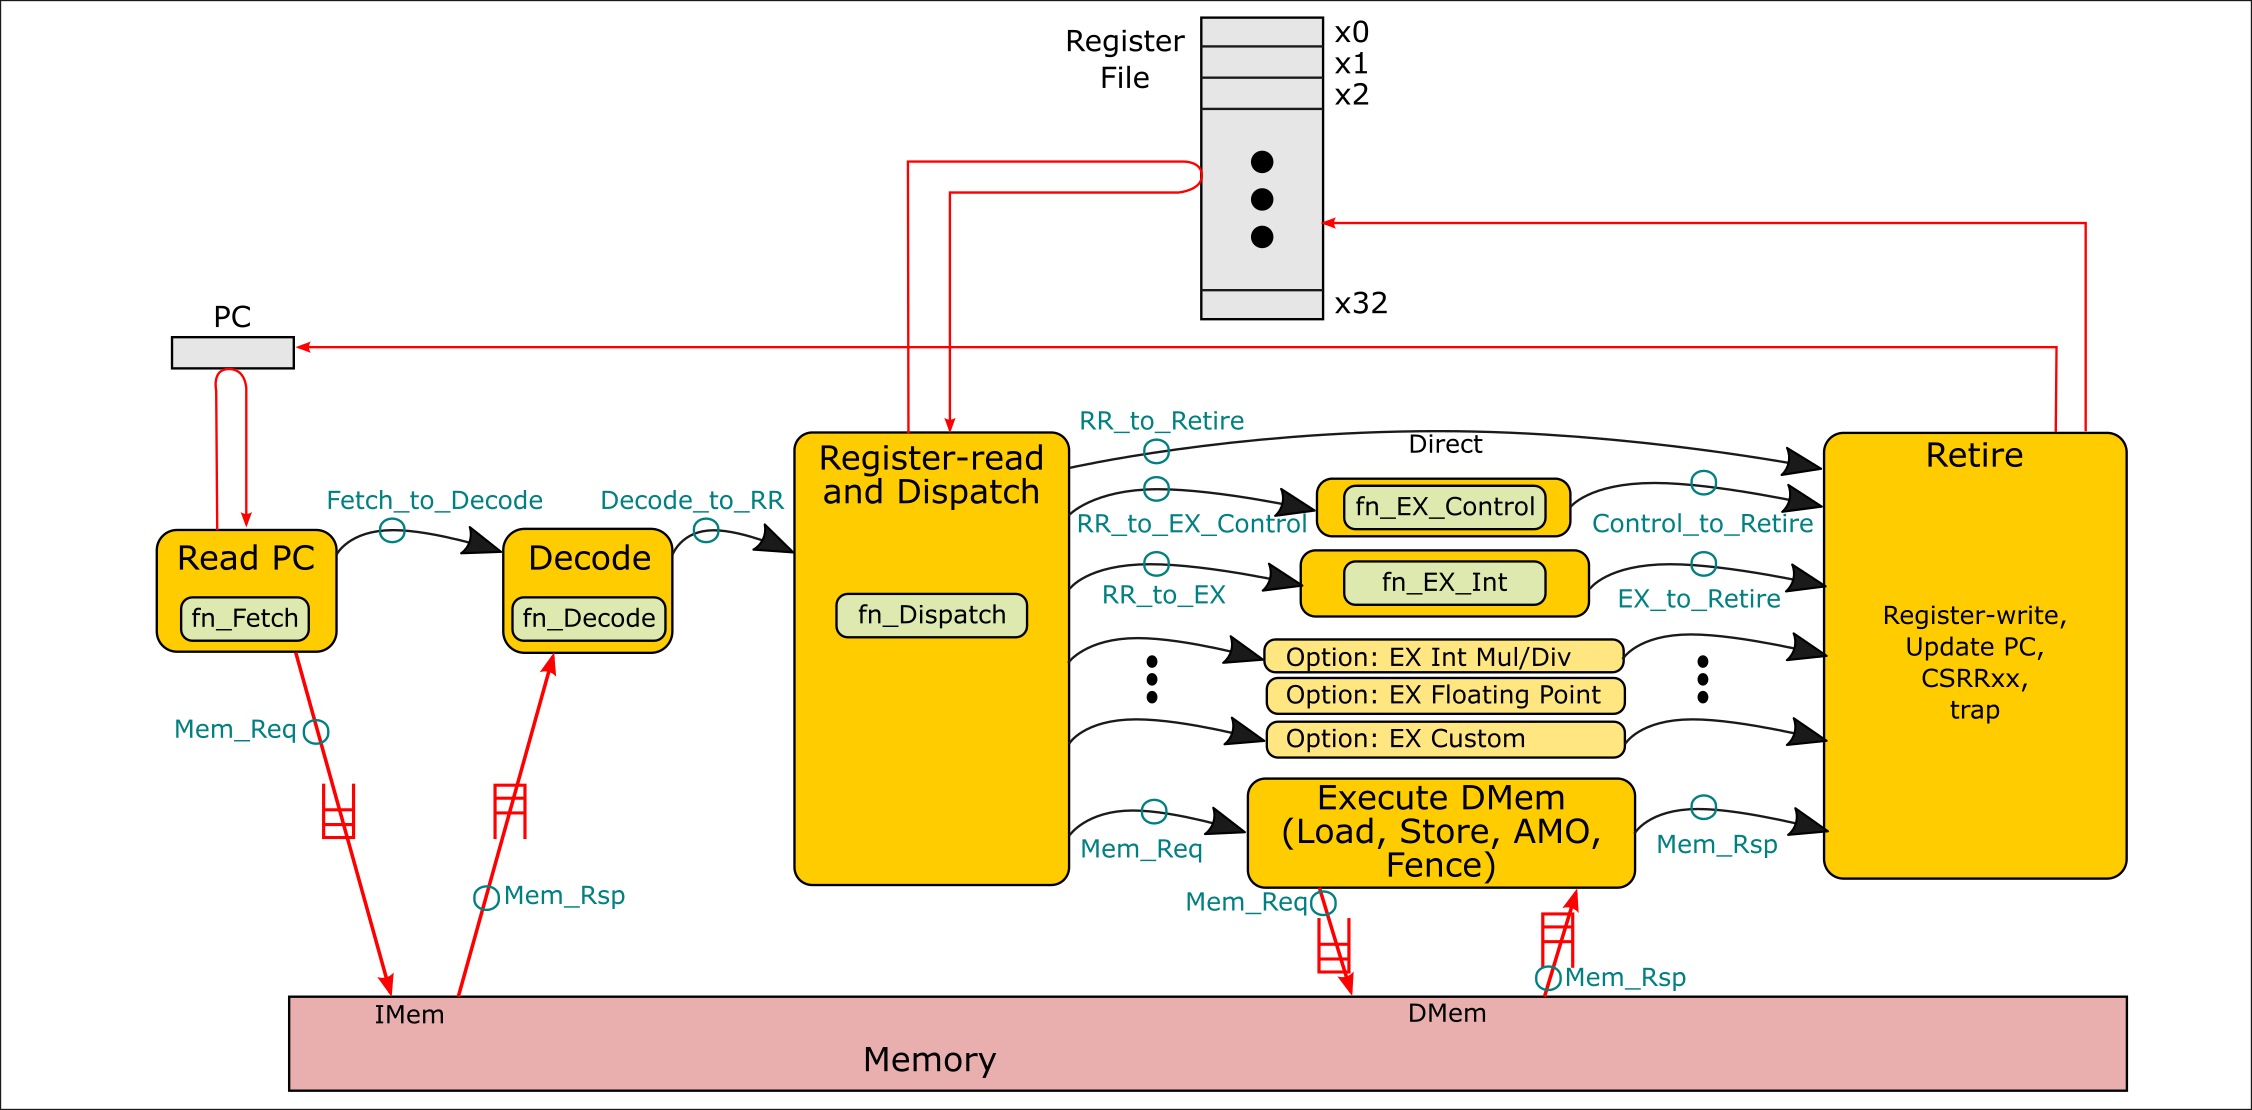
\includegraphics[height=0.6\textheight]{Fig_Instr_Exec_w_structs}
\end{center}

\end{frame}

% ================================================================

\begin{frame}
\frametitle{Table of Contents}

\tableofcontents

\end{frame}

% ****************************************************************

\section{Generic Information on Modules and Interfaces}

% ================================================================

\begin{frame}

\begin{center}
  {\LARGE Generic Information on Modules and Interfaces}
\end{center}

\end{frame}

% ================================================================

\begin{frame}
\frametitle{{\BSV}: What's in an Interface Declaration?}

\begin{center}
\includegraphics[width=\textwidth]{../Figures/Fig_BSV_whats_in_an_interface_decl}
\end{center}

\end{frame}

% ================================================================

\begin{frame}
\frametitle{{\BSV}: What's in a Module Declaration?}

\begin{center}
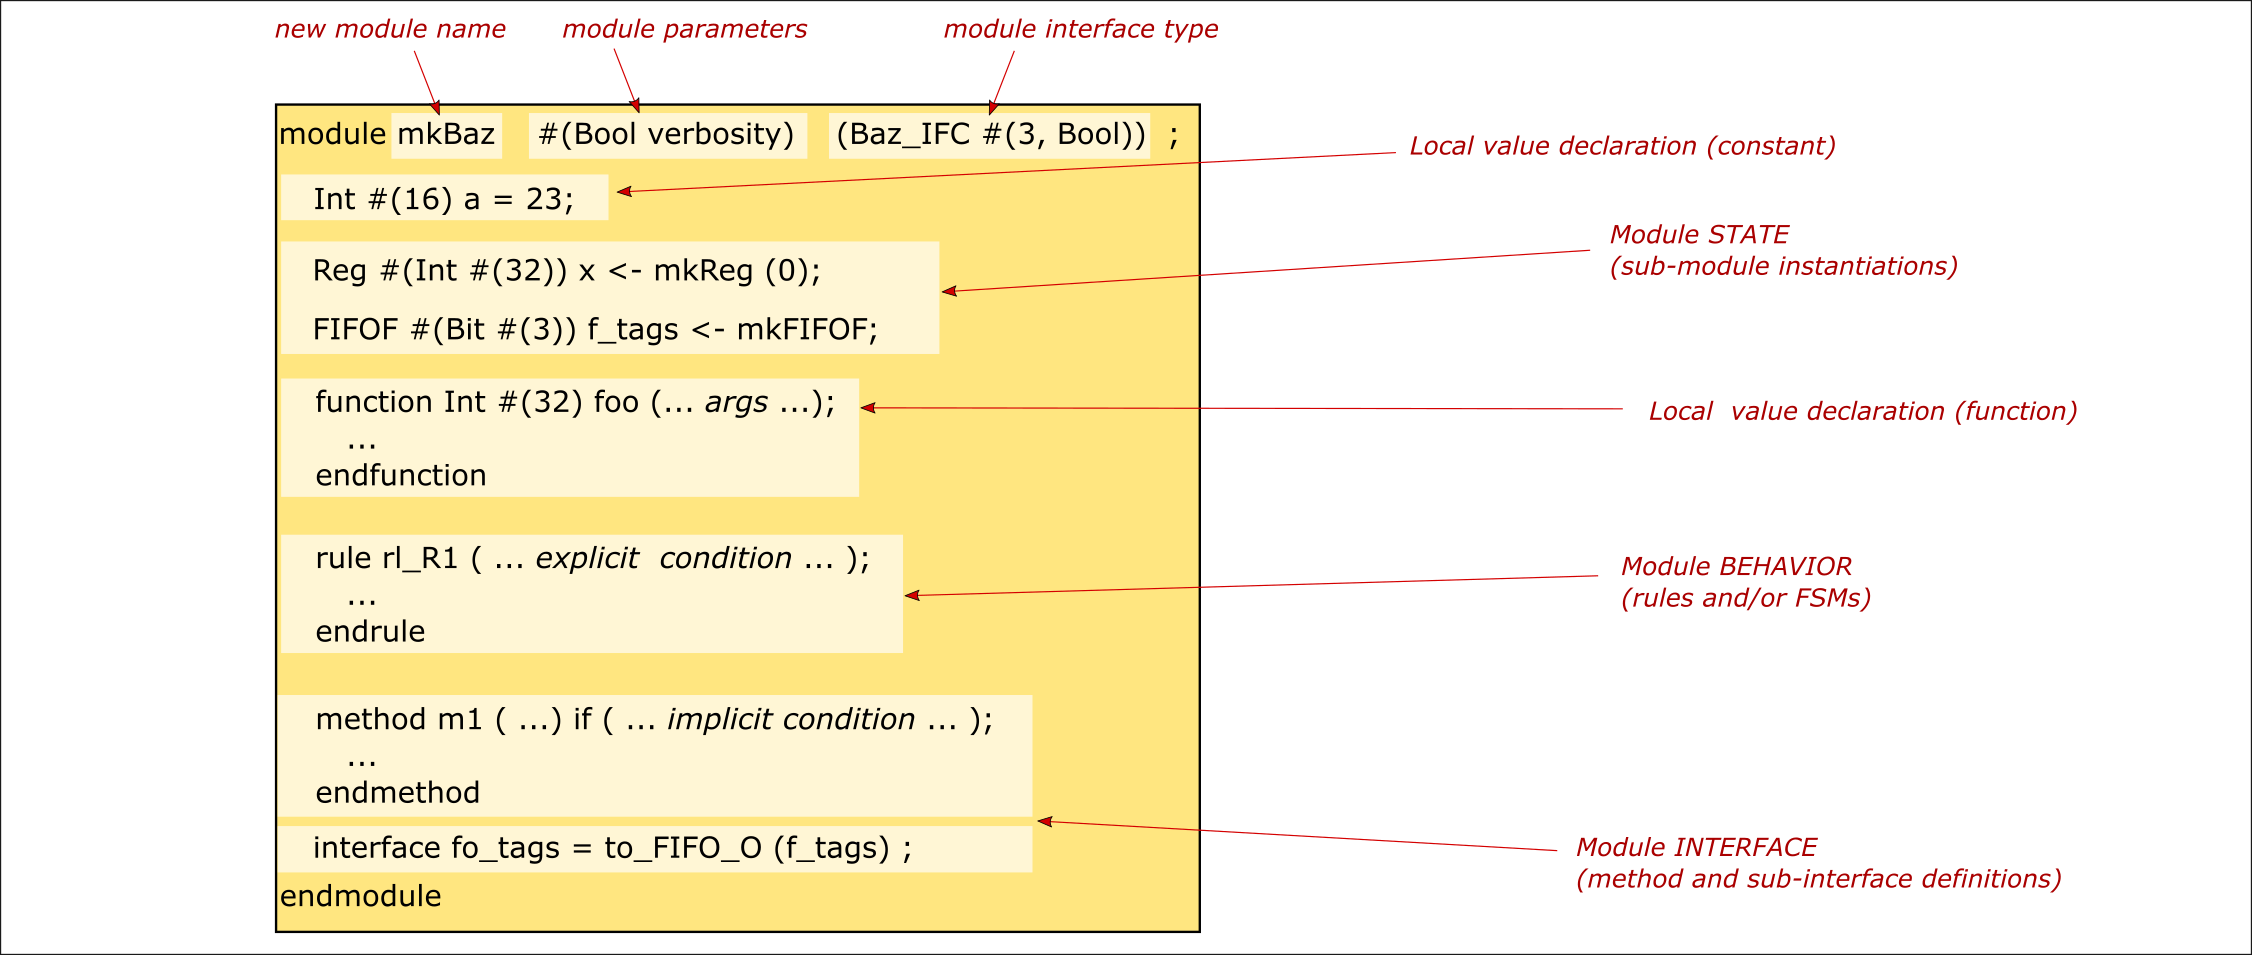
\includegraphics[width=\textwidth]{../Figures/Fig_BSV_whats_in_a_module_decl}
\end{center}

\end{frame}

% ================================================================

\begin{frame}
\frametitle{{\BSV}: What's in a Rule?}

\begin{center}
\includegraphics[width=\textwidth]{../Figures/Fig_BSV_whats_in_a_rule}
\end{center}

\end{frame}

% ================================================================

\begin{frame}
\frametitle{{\BSV}: What's in an Interface Definition?}

\begin{center}
\includegraphics[width=\textwidth]{../Figures/Fig_BSV_whats_in_an_interface_def}
\end{center}

\end{frame}

% ================================================================

\begin{frame}
\frametitle{{\BSV}: Static elaboration}

\begin{center}
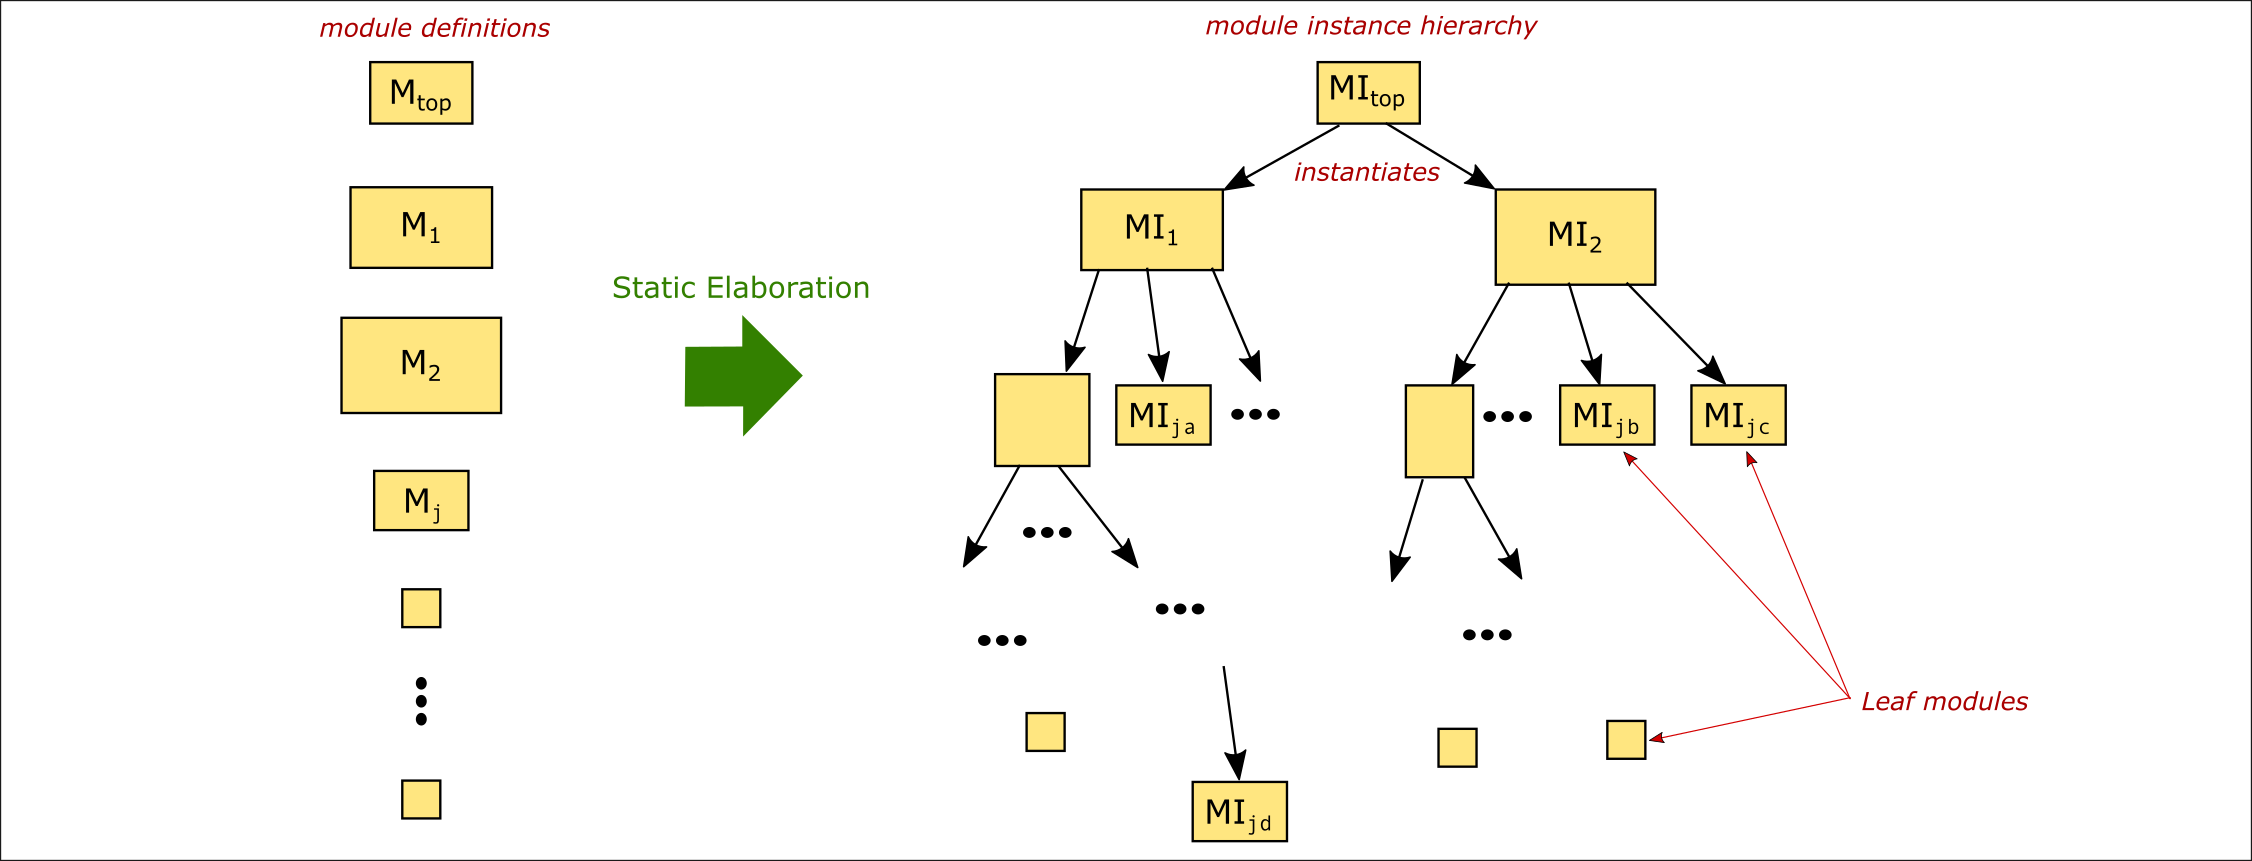
\includegraphics[width=\textwidth]{../Figures/Fig_BSV_static_elaboration}
\end{center}

\end{frame}

% ================================================================

\begin{frame}
\frametitle{{\BSV}: Module interaction}

\begin{center}

\includegraphics[width=\textwidth]{../Figures/Fig_BSV_module_interaction}
\end{center}

\end{frame}

% ================================================================

\begin{frame}[fragile]
\frametitle{{\BSV}: Generating a Verilog module for a {\BSV} module}

\footnotesize

By default, wherever we have an instantiation of a module FOO, the
{\bsc} compiler \emph{inlines} the corresponding FOO module definition
at that place.  As a consequence, there will be no trace of module FOO
in the generated Verilog.

\vspace{4ex}

We can place a ``\verb|(* synthesize *)|'' attribute just before a module declaration:

\begin{Verbatim}[frame=single]
(* synthesize *)
module mkCPU (CPU_IFC);
   ...
endmodule
\end{Verbatim}

\begin{itemize}
 \item Makes the {\bsc} compiler generate a Verilog module for {\tt mkCPU}.

 \item Wherever {\tt mkCPU} is instantiated, {\bsc} will instantiate
       that Verilog module there, instead of inlining it.

\end{itemize}

\vspace{2ex}

CAVEAT: all {\BSV} modules can be inlined, but not all {\BSV} modules
can be converted into Verilog:
\begin{itemize}

 \item The inputs and outputs of a Verilog module are all wires, carrying bit-vectors.

 \item In {\BSV}, a parameter/result of a module may have a type with
       no bit-vector representation; for example, the {\tt Integer}
       type (unbounded mathematical integers).  Inlining this module
       may reveal that this parameter is used in a way that does not
       need a bit-vector.
\end{itemize}

\end{frame}

% ================================================================

\begin{frame}
\frametitle{{\BSV}: Hardware interfaces}

\footnotesize

General hardware scheme for each {\BSV} method, depending on its output type:

\begin{center}
\includegraphics[width=\textwidth]{Fig_Interface_Buses}
\end{center}

\begin{itemize}

 \item All methods have an output READY signal.  The method can be
       invoked only when READY=1.

 \item Side-effecting methods (output types {\tt Action}, {\tt
       ActionValue \#($t$)}) have an input ENABLE signal.  The
       side-effect only occurs on clock edges when ENABLE=1.

 \item A method argument is an input bus.
 \item A method result is an output bus.
\end{itemize}

READY/ENABLE signaling is fundamental for implementing {\BSV}'s
compositional rule-based behavioral semantics (rule conditions, method
conditions, rule atomicity).

\end{frame}

% ================================================================

\begin{frame}
\frametitle{{\BSV}: Hardware interfaces: modeling Verilog/SystemVerilog ports}

\footnotesize

One can attach \emph{attributes} ``{\tt always\_ready}'' and ``{\tt
always\_enabled}'' to a {\BSV} method, eliminating the READY and/or
ENABLE signals, respectively (see documentation).

\vspace{1ex}

Note: the {\bsc} compiler will check that these attribute-assertions are true.

\vspace{4ex}

It is easy to model Verilog/SystemVerilog module ports:
\begin{itemize}

 \item A {\BSV} method with 0 arguments (no inputs) and 1 result
       (output bus) that is always-ready becomes a simple
       Verilog/SystemVerilog output port.

 \item A {\BSV} {\tt Action} method (no output) with 1 argument (input
       bus), that is always-ready and always-enabled becomes a simple
       Verilog/SystemVerilog input port.
\end{itemize}

These are frequently used for {\BSV} modules that must interface with
external Verilog/SystemVerilog IP.

\end{frame}

% ****************************************************************

\section{Registers}

% ================================================================

\begin{frame}

\begin{center}
  {\LARGE Registers}
\end{center}

\end{frame}

% ================================================================

\begin{frame}[fragile]
\frametitle{{\BSV} library: Registers}

\footnotesize

Registers are the simplest ``state elements'' (entities that have
state, {\ie} that store or retain values over time).

\vspace{2ex}

In {\BSV}, registers are just pre-defined modules. \\
(In Verilog/System Verilog, registers are special primitives, not modules.)

\vspace{2ex}

The pre-defined ``{\tt Reg}'' interface is an interface with two methods:

\begin{Verbatim}[frame=single]
interface Reg #(t);
   method t _read();
   method Action _write (t x);
endinterface
\end{Verbatim}

\vspace{1ex}


``{\tt mkReg}'' and ``{\tt mkRegU}'' are pre-defined {\BSV} modules
for registers (instantiated just like user-defined modules).

Examples:

\begin{Verbatim}[frame=single]
   Reg #(Bit #(XLEN))  rg_pc <- mkReg (0);    // 0 is the reset value

   Reg #(Bit #(XLEN))  rg_pc <- mkRegU;       // unspecified reset value
\end{Verbatim}

\vspace{2ex}

{\BSV} registers are strongly-typed. \\
A \verb|Reg #(Bit #(XLEN))| cannot contain a {\tt Bool} value,
  or a \verb|Mem_Req| value,
  or ... any value whose type is not \verb|Bit #(XLEN)| \\
(unlike Verilog/System Verilog, where all registers just hold bit-vectors).

\end{frame}

% ================================================================

\begin{frame}[fragile]
\frametitle{{\BSV}: Syntactic shorthands for reading and writing registers}

\footnotesize

Because register access is so frequent, {\BSV} provides some syntactic
shorthands for regsiter-method invocations:

\vspace{2ex}

\begin{center}
 \begin{minipage}{0.25\textwidth}
  \begin{Verbatim}[frame=single]
  rg_pc + 4
  \end{Verbatim}
 \end{minipage}
 \hm is shorthand for \hm
 \begin{minipage}{0.35\textwidth}
  \begin{Verbatim}[frame=single]
  rg_pc._read + 4
  \end{Verbatim}
 \end{minipage}

 \begin{minipage}{0.25\textwidth}
  \begin{Verbatim}[frame=single]
  rg_pc <= v
  \end{Verbatim}
 \end{minipage}
 \hm is shorthand for \hm
 \begin{minipage}{0.35\textwidth}
  \begin{Verbatim}[frame=single]
  rg_pc._write (v);
  \end{Verbatim}
 \end{minipage}
\end{center}

\PAUSE{\vspace{4ex}}

Example:

\vspace{1ex}

\begin{center}
 \begin{minipage}{0.25\textwidth}
  \begin{Verbatim}[frame=single]
  rg_pc <= rg_pc + 4;
  \end{Verbatim}
 \end{minipage}
 \hm is shorthand for \hm
 \begin{minipage}{0.35\textwidth}
  \begin{Verbatim}[frame=single]
  rg_pc._write (rg_pc._read + 4);
  \end{Verbatim}
 \end{minipage}
\end{center}

\end{frame}

% ****************************************************************

\section{Register Files}

% ================================================================

\begin{frame}

\begin{center}
  {\LARGE Register Files}
\end{center}

\end{frame}

% ================================================================

\begin{frame}[fragile]
\frametitle{{\BSV} library: Register Files}

\footnotesize

A Register File module is an array of $n$ registers.

\vspace{4ex}

Unlike a collection of $n$ individual registers, where we can
simultaneously read and write all of them, a register file is
organized and accessed like a memory, through a read and write
interface.

\vspace{2ex}

\begin{itemize}

 \item To read the $j^{th}$ register, we must give it the register
       index $j$ (like a ``memory address'').

       The standard {\BSV} register file module has 5 read-ports,
       {\ie} up to 5 registers can be read simultaneously (no matter
       how many registers are in the register file).

       Note: in RISC-V, we need to read rs1 and rs2 simultaneously.

 \PAUSE{\vspace{2ex}}

 \item To write the $j^{th}$ register, we must give it the register
       index $j$ and the value $v$ to be written.

\end{itemize}

\PAUSE{\vspace{2ex}}

A synthesis tool might implement a register file using an SRAM,
instead of individual registers and muxes.

\end{frame}

% ================================================================

\begin{frame}[fragile]
\frametitle{{\BSV} library: Register Files}

\footnotesize

(See ``Bluespec Compiler (BSC) Libraries Reference Guide'', Section ``3.1.1 Register File''.)

\vspace{2ex}

The {\tt RegFile} interface:

\begin{Verbatim}[frame=single]
interface RegFile #(type index_t, type data_t);
   method Action upd (index_t addr, data_t d);      // write a register
   method data_t sub (index_t addr);                // read a register
endinterface: RegFile
\end{Verbatim}

``\verb|index_t|'' is the type for the index (for RISC-V, with 32
registers, we use \verb|Bit#(5)|).

``\verb|data_t|'' is the type of value stored in each of the
registers (for RISC-V, this is \verb|Bit#(XLEN)|.

\vspace{2ex}

{\BSV} register files are strongly typed, just like individul registers. \\
(In Verilog/SystemVerilog, where register files just hold bit-vectors.)

\vspace{2ex}

``{\tt mkRegFile}'' and ``{\tt mkRegFileFull}'' are pre-defined {\BSV}
modules for register files (instantiated just like user-defined
modules).

Examples:

\begin{Verbatim}[frame=single]
RegFile #(Bit #(5), Bit #(XLEN)) gprs <- mkRegFile (1, 31);    // 31 registers; addrs 1..31

RegFile #(Bit #(5), Bit #(XLEN)) gprs <- mkRegFileFull;        // 32 registers; addrs 0..31
\end{Verbatim}

\end{frame}

% ****************************************************************

\section{FIFOs}

% ================================================================

\begin{frame}

\begin{center}
  {\LARGE FIFOs}
\end{center}

\end{frame}

% ================================================================

\begin{frame}[fragile]
\frametitle{{\BSV} library: FIFOs}

\footnotesize

FIFO modules hold \emph{queues} of items. \\
We can \emph{enqueue} an item on one end of a FIFO. \\
At the other end of the FIFO, we can examine the first element, and/or
\emph{dequeue} (remove) an item.

\PAUSE{\vspace{2ex}}

A pre-defined FIFO interface in the {\BSV} library:
\begin{Verbatim}[frame=single]
interface FIFOF #(t);
   method Bool   notEmpty;
   method Bool   notFull;
   method t      first;
   method Action deq;
   method Action enq (t x);
   method Action clear;        // Empty the FIFO
endinterface
\end{Verbatim}

``{\tt t}'' specifies the type of the elements in the FIFO.

{\BSV} FIFOs are strongly typed.  \hmmmm {\Eg} a \verb|FIFOF #(Mem_Req)| cannot hold \verb|Mem_Rsp|s.

\vspace{4ex}

The {\tt first} and {\tt deq} methods (``output side'') are enabled
only when there is at least one item in the FIFO (it is not empty).

\vspace{1ex}

The {\tt enq} method (``input side'') is enabled only when there is space
available in the FIFO (it is not full).

\end{frame}

% ================================================================

\begin{frame}[fragile]
\frametitle{{\BSV} library: FIFO modules}

\footnotesize

``{\tt mkFIFOF}'' and ``{\tt mkSizedFIFOF}'' are pre-defined {\BSV} modules for FIFOs
(instantiated just like user-defined modules).

Examples:

\begin{Verbatim}[frame=single]
   // "small" capacity, used like single-register buffers
   FIFOF #(Mem_Req) f_to_IMem   <- mkFIFOF;
   FIFOF #(Mem_Rsp) f_from_IMem <- mkFIFOF;

   // Higher capacity
   FIFOF #(RR_to_Retire)  f_RR_to_Retire <- mkSizedFIFOF (8);
\end{Verbatim}

\end{frame}

% ================================================================

\begin{frame}[fragile]
\frametitle{{\bf RISC-V} (Fife): Balancing fork-join pipeline paths}

\footnotesize

\begin{center}
\includegraphics[height=0.5\textheight]{Fig_Instr_Exec_w_FIFOs}
\end{center}

Suppose we use a small (capacity 1) FIFO \emph{fd} on the direct path
from Fetch to Decode. After Fetch enqueues one item into \emph{fd}
and to memory, it will get stuck---\emph{fd} is full, and will remain
full until Decode receives the response from memory, when it will
dequeue \emph{fd}.

\vspace{1ex}

For Fetch to continue, \emph{fd} needs higher capacity---equal to the
number of items that may be ``in flight'' on the path to memory and
back (memory requests, IMem, memory-responses).  In other words, the
two paths must be ``balanced''.

\end{frame}

% ================================================================

\begin{frame}[fragile]
\frametitle{{\BSV} library: A useful help-function}

\footnotesize

A useful function combining the {\tt first} and {\tt deq} methods:
\begin{Verbatim}[frame=single]
function ActionValue #(t) pop (FIFOF #(t) fifo);
   actionvalue
      let x = fifo.first;
      fifo.deq;
      return x;
   endactionvalue
endfunction
\end{Verbatim}

\vspace{4ex}

\begin{center}
So \hmm
\begin{minipage}{0.3\textwidth}
\begin{Verbatim}[frame=single]
   let y <- pop (fifo);
\end{Verbatim}
\end{minipage}
\hmm is equivalent to \hmm
\begin{minipage}{0.3\textwidth}
\begin{Verbatim}[frame=single]
   let y fifo.first;
   fifo.deq;
\end{Verbatim}
\end{minipage}
\end{center}

\end{frame}

% ================================================================

\begin{frame}[fragile]
\frametitle{{\BSV} library: {\tt SemiFIFOF} interfaces for each end of a FIFO}

\footnotesize

When a FIFO is used for communication between two modules, it is
enqueued in one module and dequeued in the other.  Conceptually, each
module uses only one end of the FIFO.

\vspace{1ex}

For this, it is useful to define interfaces representing one end of a FIFO:

\vspace{1ex}

Input end (where we enqueue):
\begin{Verbatim}[frame=single]
interface FIFOF_I #(t);
   method Bool notFull();
   method Action enq (t x);
endinterface
\end{Verbatim}

\vspace{1ex}

Output end (where we dequeue), and associated \verb|pop_O| function:

\begin{minipage}[t]{0.3\textwidth}
\begin{Verbatim}[frame=single]
interface FIFOF_O #(t);
   method Bool notEmpty();
   method t first();
   method Action deq();
endinterface
\end{Verbatim}
\end{minipage}
\hm
\begin{minipage}[t]{0.6\textwidth}
\begin{Verbatim}[frame=single]
function ActionValue #(t) pop_O (FIFOF_O #(t) fo);
   actionvalue
      let x = fo.first;
      fo.deq;
      return x;
   endactionvalue
endfunction
\end{Verbatim}
\end{minipage}

\end{frame}

% ================================================================

\begin{frame}[fragile]
\frametitle{{\BSV} library: transforming a {\tt FIFOF} interface into a {\tt FIFOF\_O} interface}

\footnotesize

\begin{Verbatim}[frame=single]
function FIFOF_O #(t) to_FIFOF_O (FIFOF #(t) f);
   interface FIFOF_O #(Mem_Req) fo_IMem_req;
      method Bool notEmpty();
         return f.notEmpty;
      endmethod

      method t first();
         return f.first;
      endmethod

      method Action deq();
         f.deq;
      endmethod
   endinterface
endfunction
\end{Verbatim}

\PAUSE{\vspace{4ex}}

We can write a similar function transforming a {\tt FIFOF} interface
into a {\tt FIFOF\_I} interface.

\end{frame}

% ================================================================

\begin{frame}
\frametitle{\EmojiExercise \hmm Exercise break}

Please see Appendix E, Exercise Ex-07-A-Interface-Transformers.

\end{frame}

% ================================================================

\begin{frame}[fragile]
\frametitle{{\BSV} library: Connecting FIFOs}

\footnotesize

\begin{center}
\begin{minipage}{0.4\textwidth}
\begin{Verbatim}[frame=single]
interface Fetch_IFC;
   interface FIFOF_O #(F_to_D)
             fo_Fetch_to_Decode;
   ...
endinterface
\end{Verbatim}
\end{minipage}
\hmm
\begin{minipage}{0.4\textwidth}
\begin{Verbatim}[frame=single]
interface Decode_IFC;
   interface FIFOF_I #(F_to_D)
             fi_Fetch_to_Decode;
   ...
endinterface
\end{Verbatim}
\end{minipage}
\end{center}

\vspace{2ex}

In the parent CPU module:

\begin{Verbatim}[frame=single]
module mkCPU (CPU_IFC);
   ...
   // Instantiate Fetch and Decode stages
   Fetch_IFC   stage_F  <- mkFetch;
   Decode_IFC  stage_D  <- mkDecode;
   ...
   // Connect the Fetch_to_Decode flow
   Empty eifc <- mkConnection (stage_F.fo_Fetch_to_Decode, stage_D.fi_Fetch_to_Decode);
   ...
endmodule
\end{Verbatim}

\end{frame}

% ================================================================

\begin{frame}[fragile]
\frametitle{{\BSV} library: {\tt mkConnection}}

\footnotesize

{\tt mkConnection} is just another module, and could easily be written
by the user if it were not pre-defined for the \verb|FIFOF_O| and
\verb|FIFOF_I| interfaces.

\begin{Verbatim}[frame=single]
module mkConnection #(FIFOF_O #(Fetch_to_Decode) f,    // module argument
                      FIFOF_I #(Fetch_to_Decode) d)    // module argument
                    (Empty);                           // module interface
   rule rl_connect;
       let x = f.first;
       f.deq;
       d.enq (x);
   endrule
endmodule
\end{Verbatim}

\PAUSE{\vspace{4ex}}

In general, whenever there is pair of interface types that can and are
frequently connected, we recommend defining {\tt mkConnection} for
those interfaces.

\end{frame}

% ================================================================

\begin{frame}[fragile]
\frametitle{{\BSV} library: {\tt mkConnection}}

\footnotesize

Shorthand: in this line:

\vspace{1ex}

\begin{Verbatim}[frame=single]
   Empty eifc <- mkConnection (stage_F.fo_Fetch_to_Decode, stage_D.fi_Fetch_to_Decode);
\end{Verbatim}

\vspace{1ex}

Because this is an empty interface (has no methods) and is therefore
never used, in {\BSV} we can just omit the ``{\tt Empty eifc <-}''
part:

\vspace{1ex}

\begin{Verbatim}[frame=single]
   mkConnection (stage_F.fo_Fetch_to_Decode, stage_D.fi_Fetch_to_Decode);
\end{Verbatim}

\end{frame}

% ================================================================

\begin{frame}[fragile]
\frametitle{{\BSV}: FIFO connections between separately compiled modules}

\footnotesize

\begin{minipage}{0.34\textwidth}
We frequently use the following scheme to make a FIFO connection
between separately compiled modules:
\end{minipage}
\hfill
\begin{minipage}{0.64\textwidth}
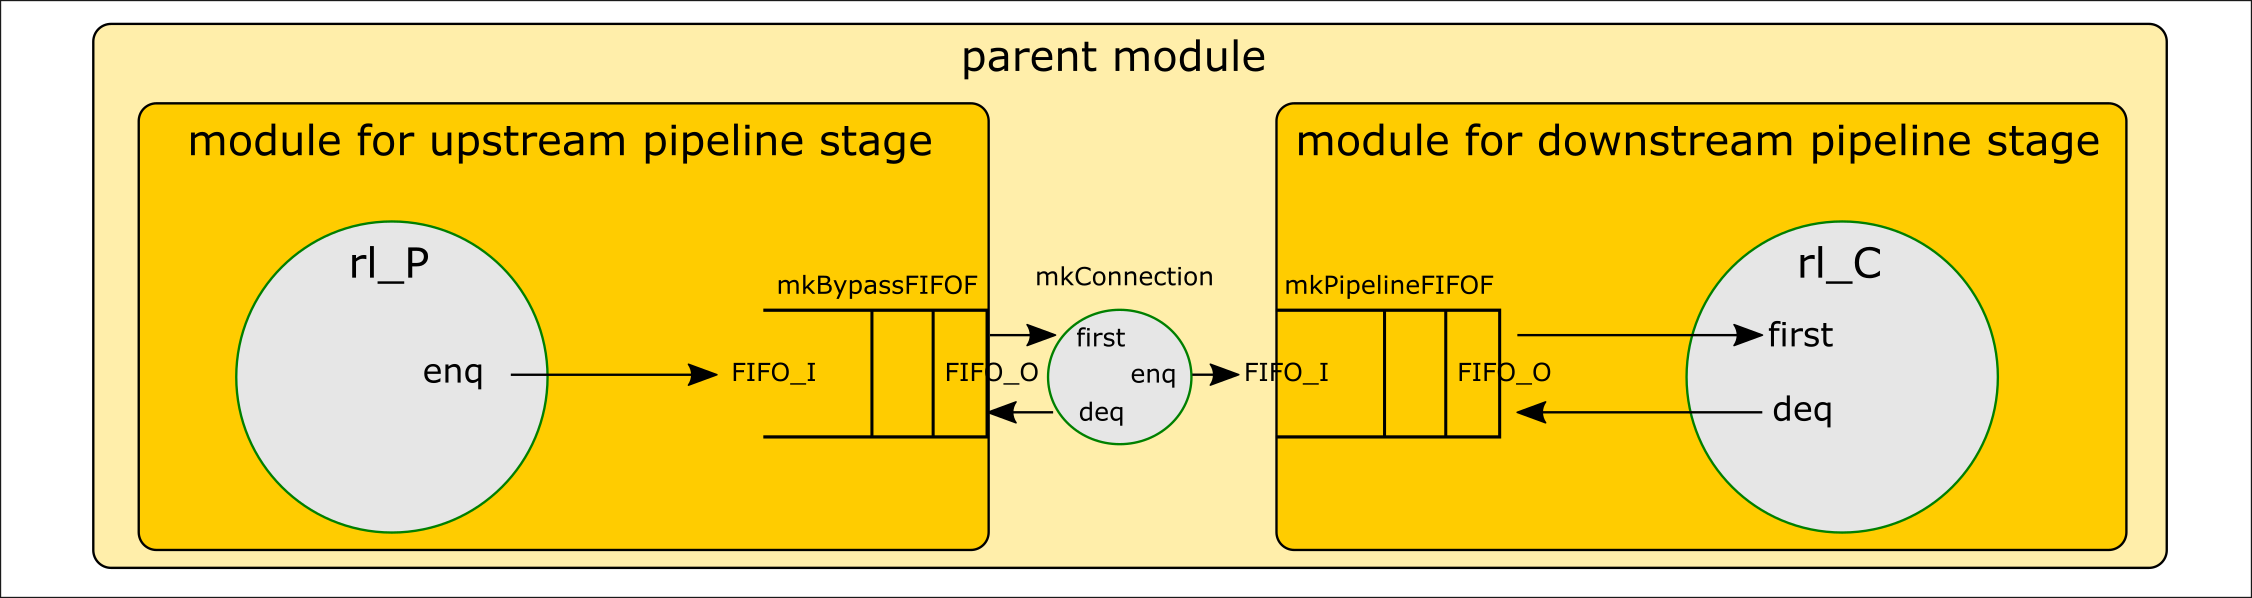
\includegraphics[width=\textwidth]{Fig_Composed_FIFO_modularity}
\end{minipage}

\PAUSE{\vspace{2ex}}

The ``modularity'' benefits are discussed in the book, Section 17.5.  Briefly:

\begin{itemize}

 \item Despite there being two FIFOs, data can traverse from producer
       to consumer in 1 tick, as desired.

 \item The structure allows the producer and consumer to be compiled
       independently by \emph{bsc}, with no ``rule-scheduling''
       constraints leaking across stage boundaries.

 \item There are no combinational paths crossing the stage boundary
       (through the two FIFOs).

 \item The structure allows us to reason about (and prove) correctness
       of each stage completely independently of other stages.

\end{itemize}

\begin{minipage}{0.2\textwidth}
 Example: in Fife code \\
 ({\tt Code/src\_Fife/})
\end{minipage}
\fbox{
\begin{minipage}{0.75\textwidth}
 \begin{itemize}\scriptsize

  \item In {\tt S2\_Decode.bsv}, see {\tt f\_Decode\_to\_RR}
        instantiation and {\tt fo\_Decode\_to\_RR} sub-interface
        definition.

  \item In {\tt S3\_RR\_RW.bsv}, see {\tt f\_Decode\_to\_RR}
        instantiation and {\tt fi\_Decode\_to\_RR} sub-interface definition.

  \item In {\tt CPU.bsv}, \\
        \hm see instantiation of {\tt stage\_D} and {\tt stage\_RR\_RW} \\
        \hm see: {\tt mkConnection (stage\_D.fo\_Decode\_to\_RR, stage\_RR\_RW.fi\_Decode\_to\_RR)}

 \end{itemize}
\end{minipage}}

\end{frame}

% ****************************************************************

\section{Polymorphic and Monomorphic Types}

% ================================================================

\begin{frame}

\begin{center}
  {\LARGE Polymorphic and Monomorphic Types}
\end{center}

\end{frame}

% ================================================================

\begin{frame}[fragile]
\frametitle{{\BSV}: Polymorphic and Monomorpic Types}

\footnotesize

A \emph{Polymorphic Type} is a type expression containing one or more
type variables. Examples:

\vspace{1ex}

\begin{center}
 \begin{minipage}{0.6\textwidth}
  \begin{Verbatim}[frame=single]
Reg #(t)
RegFile #(index_type, content_type)    GPRs_IFC #(reg_width)
FIFOF_I #(t)
FIFOF_O #(t)
  \end{Verbatim}
 \end{minipage}
 \begin{minipage}{0.35\textwidth}
  Note: type variables begin with lower-case letter
 \end{minipage}
\end{center}

\vspace{1ex}

A \emph{Monomorphic Type} (or a \emph{concrete type} is a type
expression that does not contain any type variables.  Examples:

\vspace{1ex}

\begin{center}
 \begin{minipage}{0.6\textwidth}
  \begin{Verbatim}[frame=single]
Reg #(Bool)    Reg #(Int)    Reg #(Mem_Req)
RegFile #(Bit #(5), Bit #(32))     GPRs_IFC #(32)
FIFOF_I #(Mem_Req)
FIFOF_O #(Mem_Rsp)
  \end{Verbatim}
 \end{minipage}
 \begin{minipage}{0.35\textwidth}
  Note: all type identifiers here begin with upper-case letter
 \end{minipage}
\end{center}

\vspace{1ex}

A polymorphic type reprsents all possible types we can get by
substituting each type variable by any concrete type.

\end{frame}

% ================================================================

\begin{frame}
\frametitle{\EmojiExercise \hmm Exercise break}

Please see Appendix E, Exercise Ex-07-B-Polymorphic-Types.

\end{frame}

% ================================================================

\begin{frame}[fragile]
\frametitle{{\BSV}: Synthesizable modules}

\footnotesize

Caveat:
\fbox{
 \begin{minipage}{0.9\textwidth}
   Here we use the term ``synthesize'' to mean ``generate
   Verilog'', as opposed to in-lining.

   \vspace{1ex}

   Elsewhere, the term
   ``synthesize'' is used to mean ``from RTL, generate FPGA LUTs/ASIC gates''.
 \end{minipage}}

\vspace{5ex}

By default, a {\BSV} module is \emph{in-lined} wherever it is instantiated.

\vspace{1ex}

We can precede a {\tt module} declaration {\tt mkFoo} with ``{\tt (*
synthesize *)}'':

\begin{Verbatim}[frame=single]
   (* synthesize *)
   module mkFoo (... interface type ...)
      ...
   endmodule
\end{Verbatim}

Then, {\bsc} will do the following:
\begin{itemize}
 \item It will generate a corresponding  Verilog module {\tt mkFoo}

 \item At each place where {\tt mkFoo} is instantiated, {\bsc} will
       generate Verilog code to instantiate the Verilog module {\tt mkFoo},
       instead of in-lining.
\end{itemize}

\end{frame}

% ================================================================

\begin{frame}[fragile]
\frametitle{{\BSV}: Synthesizable modules}

\footnotesize

Not all {\BSV} modules can be synthesized into Verilog, because some
module parameter, method argument or method result may not be
representable as a fixed-width bit-vector (which is needed to map it
into a Verilog module port).

\vspace{2ex}

Example reason: \hm
\fbox{
 \begin{minipage}{0.8\textwidth}
  If a method in the {\BSV} module's interface has an argument or
  result of polymorphic type, then {\BSV} does not know what the width
  will be (and the width can be different at different instantiations
  with different concrete type).
 \end{minipage}
}

Example reason: \hm
\fbox{
 \begin{minipage}{0.8\textwidth}
  If a method in the {\BSV} module's interface has an argument
  or result of type {\tt Integer} (unbounded mathematical integers),
  then {\BSV} cannot fix a specific width for this bus.
 \end{minipage}
}

Example reason: \hm
\fbox{
 \begin{minipage}{0.8\textwidth}

  A {\BSV} module's parameter can be another {\BSV} module. {\Eg}, the
  parameter may be a particular FIFO module ({\tt mkFIFOF}, {\tt
  mkSizedFIFOF(n)}, ...) to be used inside another module.  There is
  no corresponding concept in Verilog/SystemVerilog.
 \end{minipage}
}

\vspace{1ex}

\PAUSE{\vspace{2ex}}

However, \emph{all} {\BSV} modules can be inlined, and the containing
module may be synthesizable into Verilog \\
({\eg} because a polymorphic type has become concrete at this
instance, or an {\tt Integer} parameter is now only used in a
statically resolvable context).

\PAUSE{\vspace{2ex}}

We recomend using the ``{\tt (* synthesize *)}'' attribute wherever
possible because it will make Verilog debugging easier, and can help
in downstream synthesis tools ({\eg} place and route).

\PAUSE{\vspace{2ex}}

If we have a polymorphic module, we can always make one or more
monomorphic instances of that module; each of these may then be
synthesizable into Verilog (see Section 7.6.1 in book for an example).

\end{frame}

% ================================================================

\begin{frame}
\frametitle{\EmojiExercise \hmm Exercise break}

Please see Appendix E, Exercise Ex-07-C-Synthesizable-Modules.

\end{frame}

% ****************************************************************

% -*- mode: fundamental -*-

% Slides accompanying "Learn RISC-V CPU Implementation and BSV" book
% Copyright (c) 2024 Rishiyur S. Nikhil, All Rights Reserved

% This is a postamble shared by all the slide decks

% ================================================================

\begin{frame}

\begin{center}
  {\LARGE End}
\end{center}

\end{frame}

% ================================================================


% ****************************************************************

\end{document}
